\subsection{Physics motivation}

\begin{frame}{The physics motivation of the ILC - Summary}
\ilclogo
\visible<2->{ 
\alert{\MakeUppercase{Precision measurements:}}\\
}
\visible<3->{
\begin{itemize}
\item The initial particle energy is precisely known. There are no PDFs, as the initial particles are elementary.
\item Due to the high energy resolution, peaks are now measurable that weren't measurable before. Particles with small mass difference are distinguishable.
\item c-tagging is possible because of small distance between IP and the  detectors (nano-sized beam)
\end{itemize}
}
\visible<4->{ 
\alert{\MakeUppercase{Clean environment:}}\\
}
\visible<5->{
\begin{itemize}
\item Small background and no underlying events or out-of-time pileup.
\end{itemize}
}
\visible<6->{
\alert{\MakeUppercase{Model independent:}}\\
}
\visible<7->{
\begin{itemize}
\item The reactions will be measured and reconstructed in completeness. No theoretical assumptions have to be taken into account.
\item New physics and BSM physics, which are not measurable at the LHC, are accessible.
\end{itemize}
}
\end{frame}

\begin{frame}{Comparison between ILC and LHC event displays}
\begin{center}
  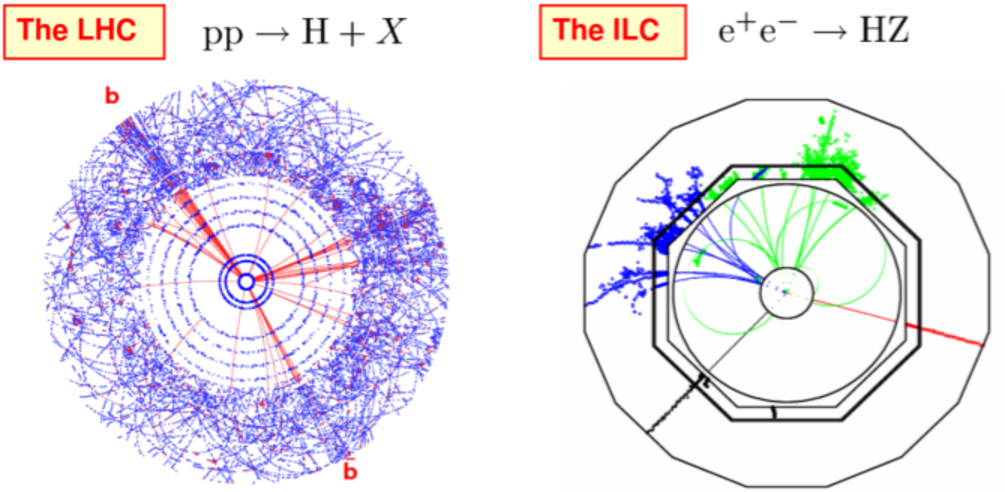
\includegraphics[width=0.75\textwidth]{figures/ILC_LHC_eventdisplay_comparison}
\end{center}
\end{frame}


